\documentclass[dvipdfmx]{jsarticle}

\usepackage{ascmac}
\usepackage{url}
\usepackage[dvipdfmx]{hyperref}
\usepackage{pxjahyper}
\usepackage[dvipdfmx]{graphicx}
\usepackage{float}
\usepackage{listings,jlisting}

\hypersetup{
  colorlinks=true,
  urlcolor=cyan,
  linkcolor=black
}

\lstset{
  basicstyle={\ttfamily},
  identifierstyle={\small},
  commentstyle={\smallitshape},
  keywordstyle={\small\bfseries},
  ndkeywordstyle={\small},
  stringstyle={\small\ttfamily},
  frame={tb},
  breaklines=true,
  columns=[l]{fullflexible},
  numbers=left,
  xrightmargin=0zw,
  xleftmargin=3zw,
  numberstyle={\scriptsize},
  stepnumber=1,
  numbersep=1zw,
  lineskip=-0.5ex
}


\begin{document}

\section{実験目的・課題}

Socket通信を行いクライアントと通信し、
クライアントから入力された成績情報を
記録するサーバプログラムを作成する。

作成するサーバーの要件
\begin{itemize}
  \item サーバープログラムとクライアントプログラムをわけて作成
  \item 接続したクライアントは何度でもメッセージのやり取りが出来る
  \item 新しく成績情報と登録できる
  \item 登録された成績情報を記録できる
  \item 今までに登録された成績情報を閲覧できる
  \item 名前か番号で検索できる
  \item 入力にエラーがある場合は通知できる
  \item 重複登録はできない
\end{itemize}


\section{実装方法}
Javaで複数のプログラム間でデータのやり取りを行うときは、
Socket通信というものを用いて通信を行う。

ここに、2つのプログラムがあり、この2つで通信を行いたいとき、
一方を「サーバー」もう一方を「クライアント」として話をする。
サーバーとクライアントは最初、何のつながりも持っていない。
ここで、サーバー側がServerSocketクラスをインスタンス化し、
その際に受け取ったポート番号の監視を始める。
次に、クライアント側でSocketクラスにサーバー名とポート番号を渡し
インスタンス化する際にサーバーに接続要求が送られる。
サーバー側ではこのSocketによる接続要求をacceptメソッドによって
受け取り、これで2つのプログラム間の接続が完了する。

\subsection{全体の方針}
今回の成績情報サーバーの作成では、サーバーとクライアントが交互に
入出力を行うことにする。
サーバーからクライアントにメッセージを送信、
それを受け取ったクライアントがそのメッセージを標準出力に出力、
それを見たユーザーがそれに対する応答をキーボードから入力する。
その入力をクライアントよりサーバーに送信し、
その入力を受けてサーバーで処理を行う。
このまとまりを処理のひとまとまりとして扱い、
これを繰り返すことで成績情報サーバーを作成する。
この処理の例を図\ref{example1}に示す。
\begin{figure}[H]
  \centering
  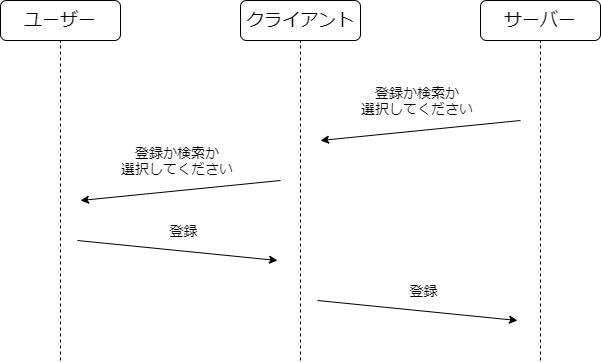
\includegraphics[width=0.7\hsize]{../pic/1.png}
  \caption{サーバーとクライアントの入出力例}
  \label{example1}
\end{figure}

クライアントプログラムでは、処理のひとまとまりを順に処理すればよいので
ソケット入力、標準出力、標準入力、ソケット出力を順に1回だけ行うコードを
whileで囲い何度もループさせればよい。

サーバープログラムでは、サーバーの要件に従い、
成績情報の登録、検索、閲覧ができるものを作成する。

\subsection{登録}
成績情報の登録にはNumber,Name,Score1\textasciitilde4が必要である。
今回はこれを一度に入力してもらうのではなく、それぞれについて
クエリを投げてそれに回答してもらう形式にする。
こうしなかった場合、例えばNumberとNameの区切り文字を
どうするかという事も決めなければならなくなるうえ、
入力にミスが含まれる可能性が高くなると考えられる。
こうしてNumberを表す文字列、Nameを表す文字列、...を得られる。
次にそれに区切り文字を付け一つの文字列になるよう連結する。
このようにして得られた文字列が正規表現に
マッチすれば入力をseisekiクラスに変換できる。



\subsection{検索}
\subsection{閲覧}


\section{結果と考察}

\begin{thebibliography}{10}
  \bibitem{1} Javaプログラムにおける通信のしくみを理解する

  \url{https://crew-lab.sfc.keio.ac.jp/lectures/2000s_mmb/JavaLectures/Lecture8/Lec8-1.html}
\end{thebibliography}
\end{document}